\section{GrainLearning evaluation}\label{section:GLPerformance} 
\begin{table}[H]
    \centering
    \begin{tabular}{l|lll|lll}
    Material                & \multicolumn{3}{l|}{Quartz Sand}       & \multicolumn{3}{l}{Limestone}          \\ \hline
    Attempt                 & 1          & 2           & 3           & 1          & 2           & 3           \\ \hline
    Restitution Coefficient & {[}0.5  1{]} & {[}0  1{]}  & {[}0 1{]}   & {[}0.5  1{]} & {[}0.5  1{]}  & {[}0 1{]}   \\
    Rolling Friction        & {[}0 1{]}  & {[}0 0.5{]} & {[}0.5 1{]} & {[}0 1{]}  & {[}0 0.5{]} & {[}0.5 1{]} \\
    Sliding Friction        & {[}0 1{]}  & {[}0 0.5{]} & {[}0.5 1{]} & {[}0 1{]}  & {[}0 0.5{]} & {[}0.5 1{]} \\
    Bond number             & {[}0 1{]}  & {[}0 0.5{]} & {[}0.5 1{]} & {[}0 1{]}  & {[}0 0.5{]} & {[}0.5 1{]} \\
    \end{tabular}
    \caption{Calibration attempts using GL}\label{table:GLCalibration}
\end{table}

Table~\ref{table:GLCalibration} gives details on different calibrations with GL for two materials mentioned above: quartz sand and limestone. The difference between each attempt is that the search range of the microparameters changed. The first attempt serves as the control for both materials, while the second and the third are set up in smaller ranges. Overall, approximately 200 DEM simulations were performed for quartz sand, and 3 produced a valid combination. For limestone, 300 DEM simulations were performed, and five are valid. The valid combinations are marked in bold on the result tables in the following section.

\subsection{Limestone}
The calibration results by GL for limestone are described in table~\ref{table:resEskalGL}, and the details on how the sampling algorithm performs, i.e., conditioned on the previous simulation, is the sampled parameters for the next iteration make the simulation result converge to the experimental result, are described in figure~\ref{fig:EskalGL}. In the third calibration attempt, the second iteration did not finish in time due to the system's high level of kinetic energy; therefore, only iteration 1 is shown. 
In the control attempt, initially, only four iterations were performed. However, one remarkable observation is that GL clusters over the combinations produce a static AoR around $40^{\circ}$. This is reflected in the second iteration's result, where the best combination results in a static AoR of $39.4803^{\circ}$. Moreover, although the third iteration's result is $33.0979^{\circ}$, this seems like an outlier of the cluster. Therefore, an additional iteration was performed~-~and the results here verify the observation. The closest value to experimental static AoR is $31.5243^{\circ}$, and it is also the outlier of the cluster. 

After the first calibration attempt, it is clear that the combinations that would result in the desired static AoR lie around $0.8-1.0$ for restitution coefficient and in the lower-0.25 range for the rest of the contact parameters. Therefore, two more attempts were performed, with different initial ranges: attempt 2 with sliding friction, rolling friction, and bond number ranging from 0 to 0.5. With attempt 3, the sliding friction, rolling friction, and bond number range from 0.5 to 1, while the restitution coefficient's range is widened to 0 to 1. 

As expected, the second attempt's performance was the most robust, reaching a near-perfect solution at the end of iteration 4. The clustering of the optimal result can also be seen clearly in figure~\ref{fig:EskalGL}. Meanwhile, the results from the third attempt verify the conclusion from the first attempt about the range of the optimal parameters~-~with higher rolling friction, sliding friction, and bond number, the static AoR reaches a maximum value of around $65^{\circ}$.



\begin{figure}[H]
    \centering
    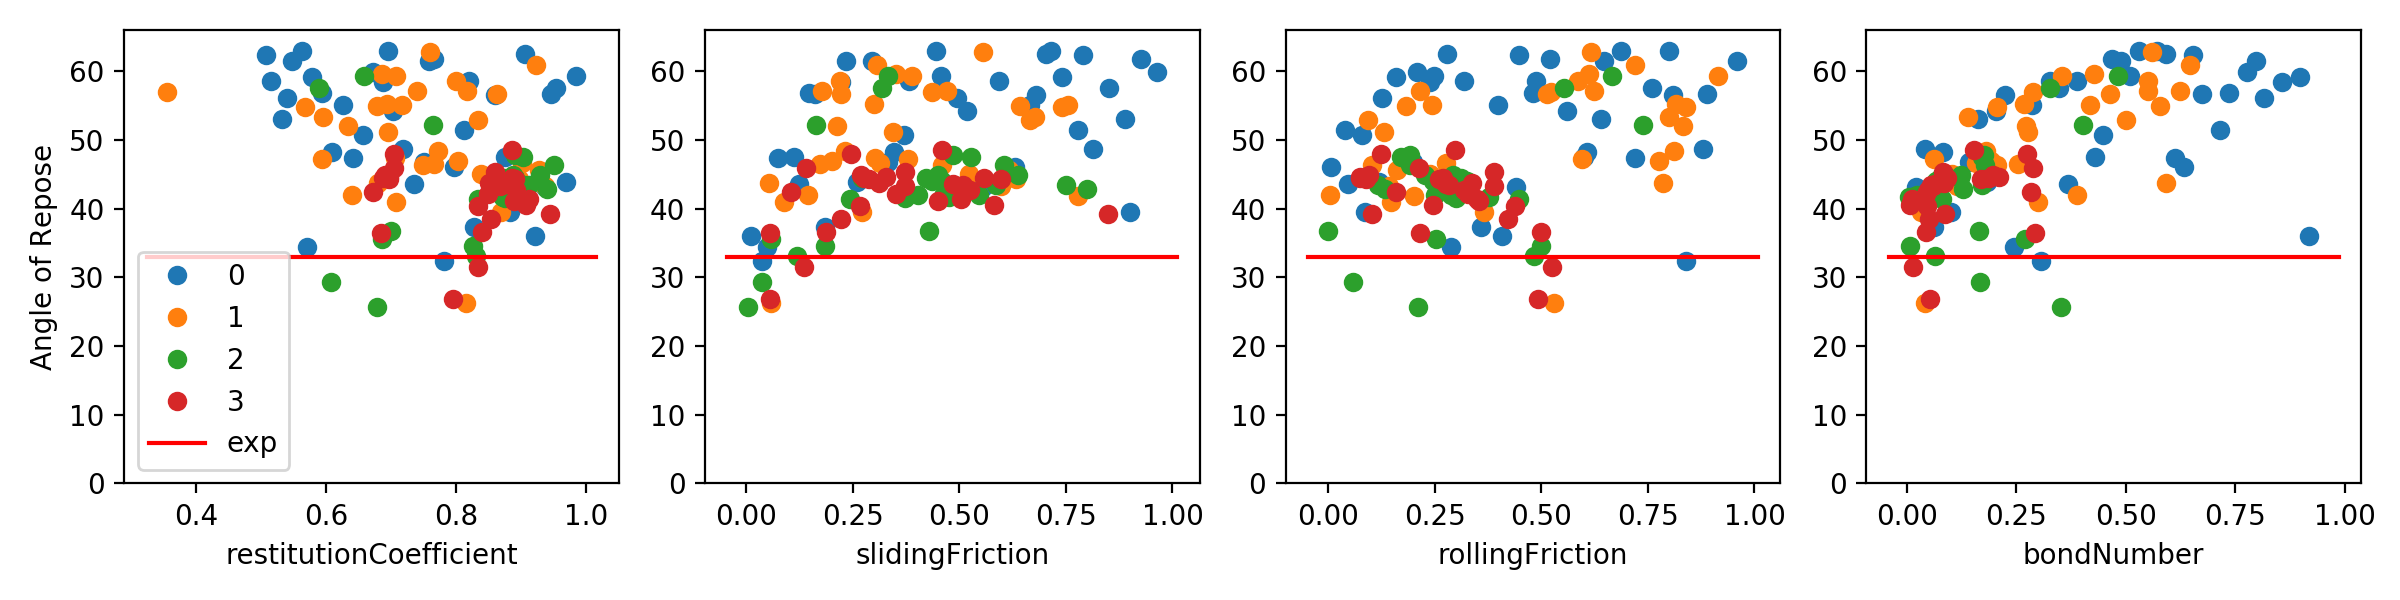
\includegraphics[scale=0.51]{ParametersObserver_Eskal150.png}
    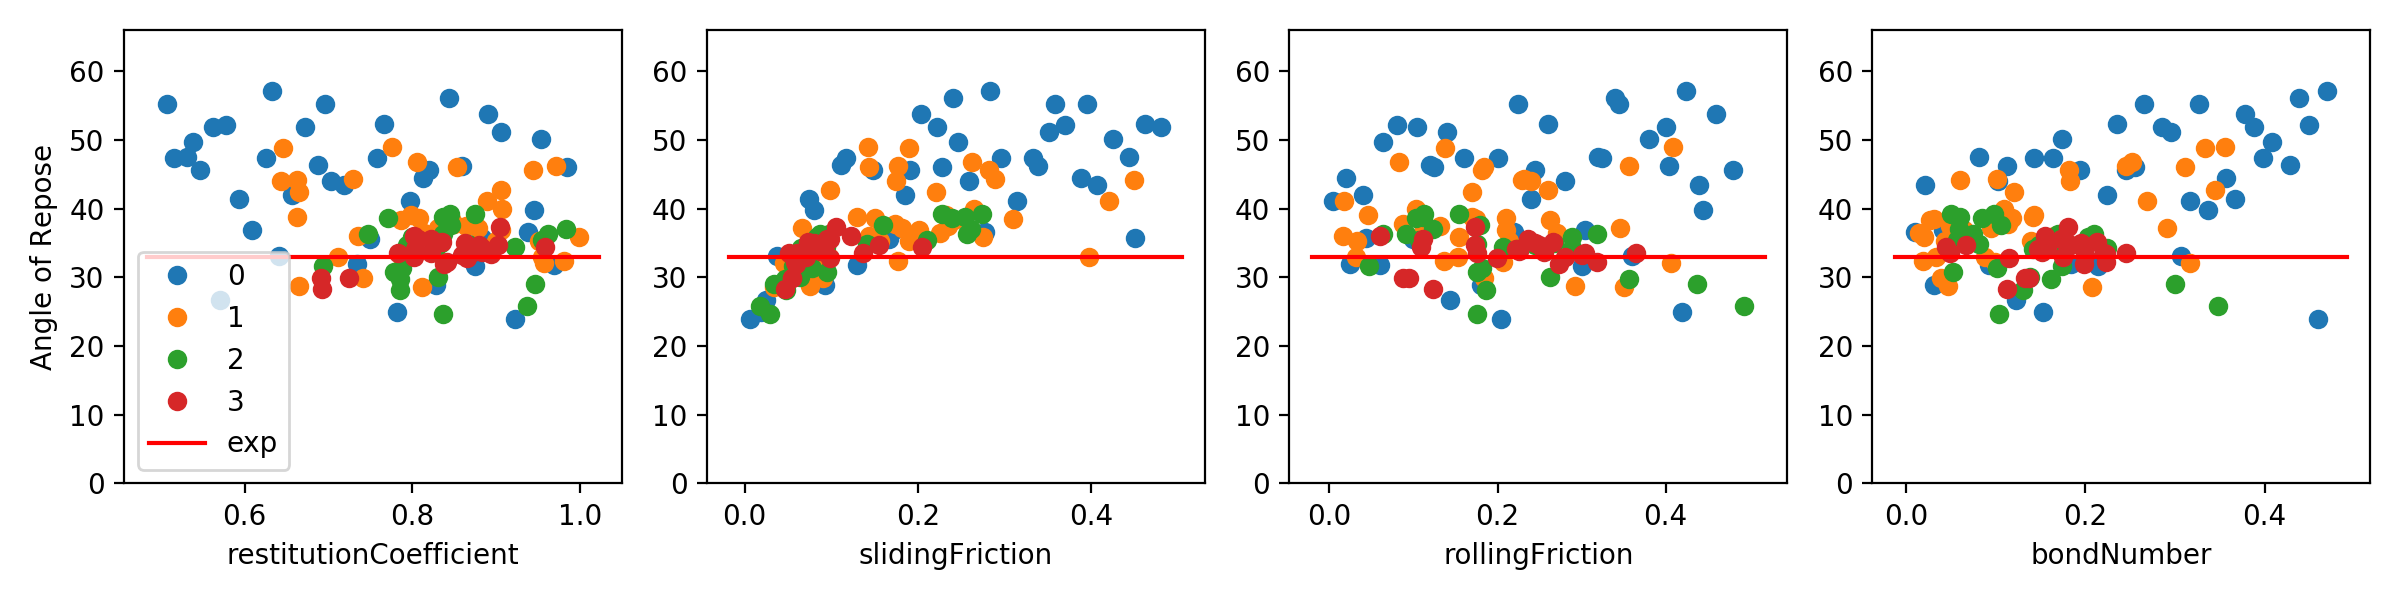
\includegraphics[scale=0.51]{ParametersObserver_Eskal150_1.png}
    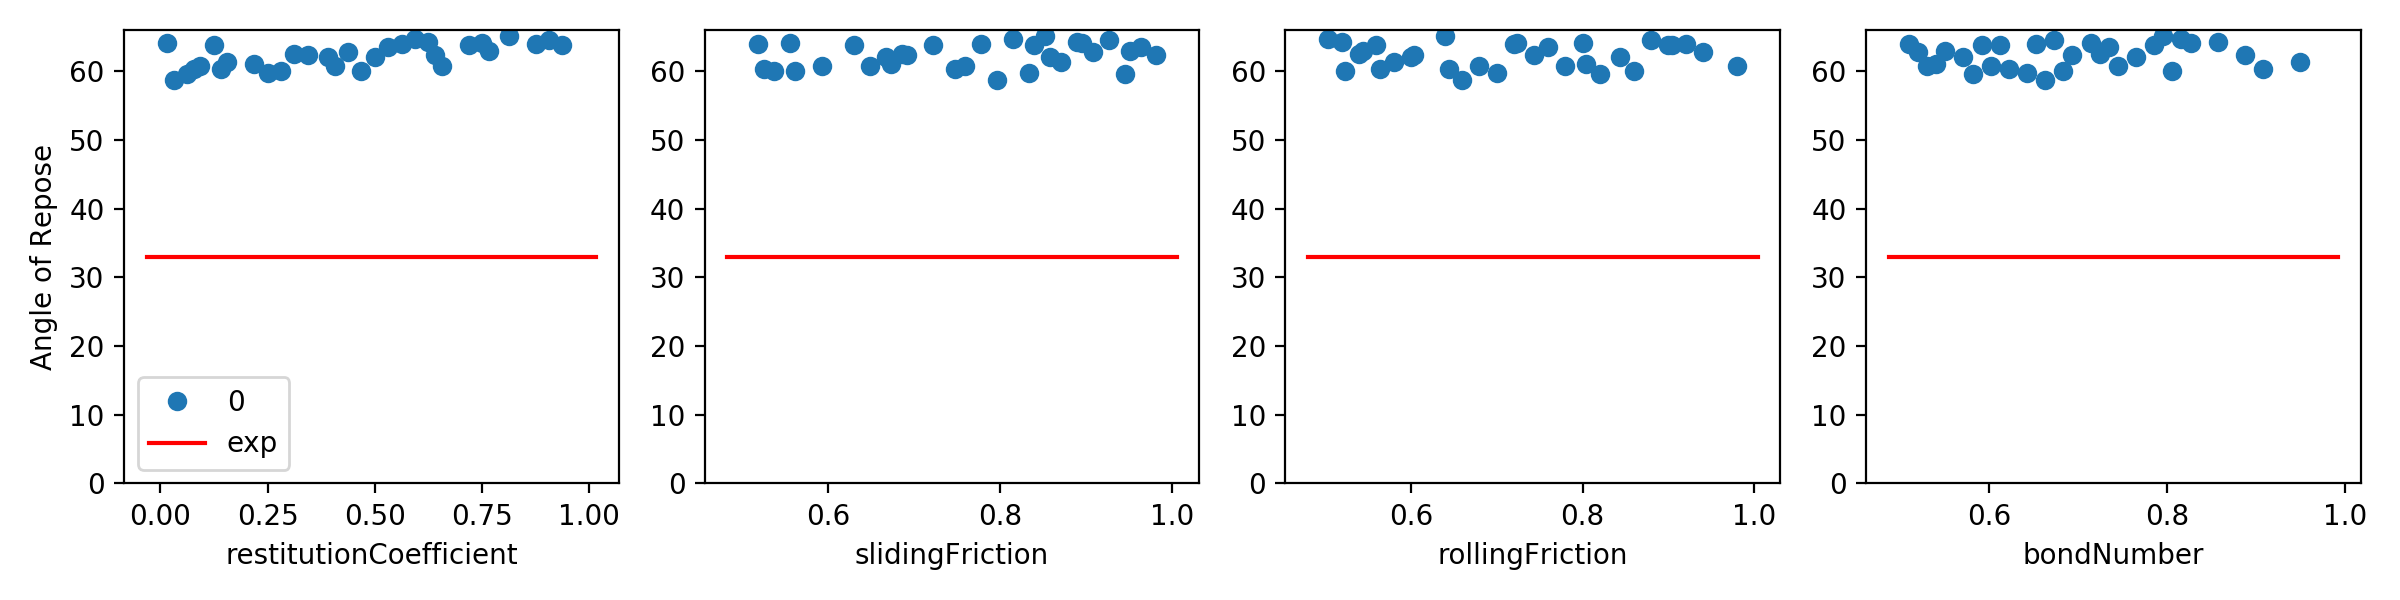
\includegraphics[scale=0.51]{ParametersObserver_Eskal150_2.png}
    \caption{\textit{From top to bottom,} attempt 1, 2, and 3 at calibrating Eskal with GL.\@ Scatter dots with different colors denote each iteration, and red line denotes experimental value.}\label{fig:EskalGL}
\end{figure}




\begin{table}[H]
    \centering
    \resizebox{\textwidth}{!}{%
    \begin{tabular}{c|ccccc}
    Attempt/Iter & Restitution Coefficient & Sliding Friction & Rolling Friction & Bond number & Result AoR \\ \hline
    1.1 & 0.7812 & 0.037 & 0.84 & 0.3061 & 32.3163 \\
    1.2 & 0.869 & 0.2725 & 0.3652 & 0.0325 & 39.4803 \\
    1.3 & 0.831 & 0.1194 & 0.484 & 0.064 & 33.0406 \\
    1.4 & 0.8332 & 0.135 & 0.5262 & 0.0137 & 31.5243 \\
    2.1 & 0.6406 & 0.037 & 0.36 & 0.3061 & 33.0979 \\
    2.2 & 0.9546 & 0.3983 & 0.032 & 0.0334 & 32.9993 \\
    2.3 & 0.8263 & 0.0917 & 0.2226 & 0.1411 & 34.1421 \\
    2.4 & 0.8025 & 0.0710 & 0.2802 & 0.1748 & 32.9812 \\
    3.1 & 0.0312 & 0.7963 & 0.66 & 0.6632 & 58.6606
    \end{tabular}%
    }
    \caption{Calibration results of limestone with GL.}\label{table:resEskalGL}
\end{table}
    

\subsection{Quartz sand}

The calibration result for quartz sand is given in table~\ref{table:resSandGL}, and the parameters sampling graph is given in figure~\ref{fig:QuartzGL}. In the control attempt, only the first iteration is shown, partly due to 6/40 simulations of the second iteration does not finish in time, but also due to the results of the second iteration does not cluster at the experimental value, with most averaging around $45^{\circ}$ to $50^{\circ}$. Due to the similarity between quartz sand and limestone in terms of experimental static AoR, the second attempt of quartz sand will be initialized with the same range as the second attempt of limestone. And as a result, attempt 2 has the best performance out of the three. One noticeable thing here is that the rolling friction has two different clusters identified by GL instead of one, compared to sliding friction, restitution coefficient, or bond number. This denotes the multi-solution phenomena of a calibration problem since there could be more than one combination that can produce a sufficient static AoR~-~which is shown in iterations 3 and 4 of attempt 2: the rolling friction for iteration 3 is 0.07, while for iteration 4 is 0.41. Different experiments, i.e., Shear Cell test or Drum test (Dynamic AoR), would be needed in addition to the heap test to find an ideal combination of microparameters. However, this is out of the scope of the current research. 

In the third attempt, although the range was specified as shown in table~\ref{table:GLCalibration}, the Gaussian Mixture Model algorithm of GL sampled some of the values in iteration 3 and 4 outside the initial range. This was a known bug in the current GL version implemented in MercuryDPM. However, it was able to generate a correct combination which results in a static AoR of $34.2227^{\circ}$, remarkably close to the experimental value, by sampling a combination with very low sliding friction. 


\begin{figure}[H]
    \centering
    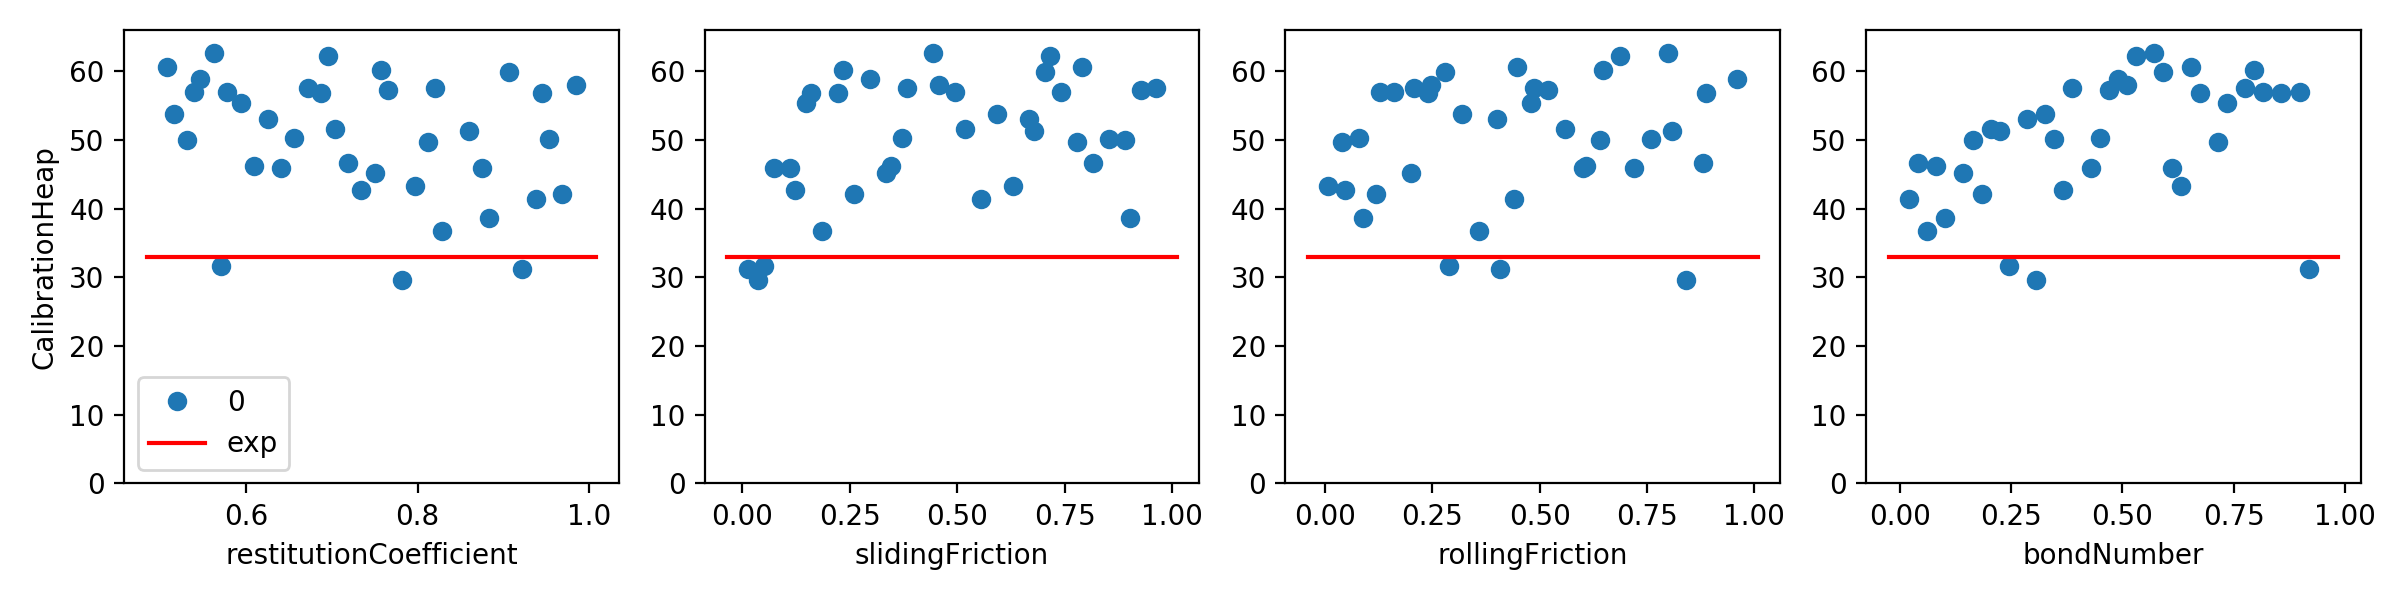
\includegraphics[scale=0.51]{ParametersObserver_SandHeap_copy.png}
    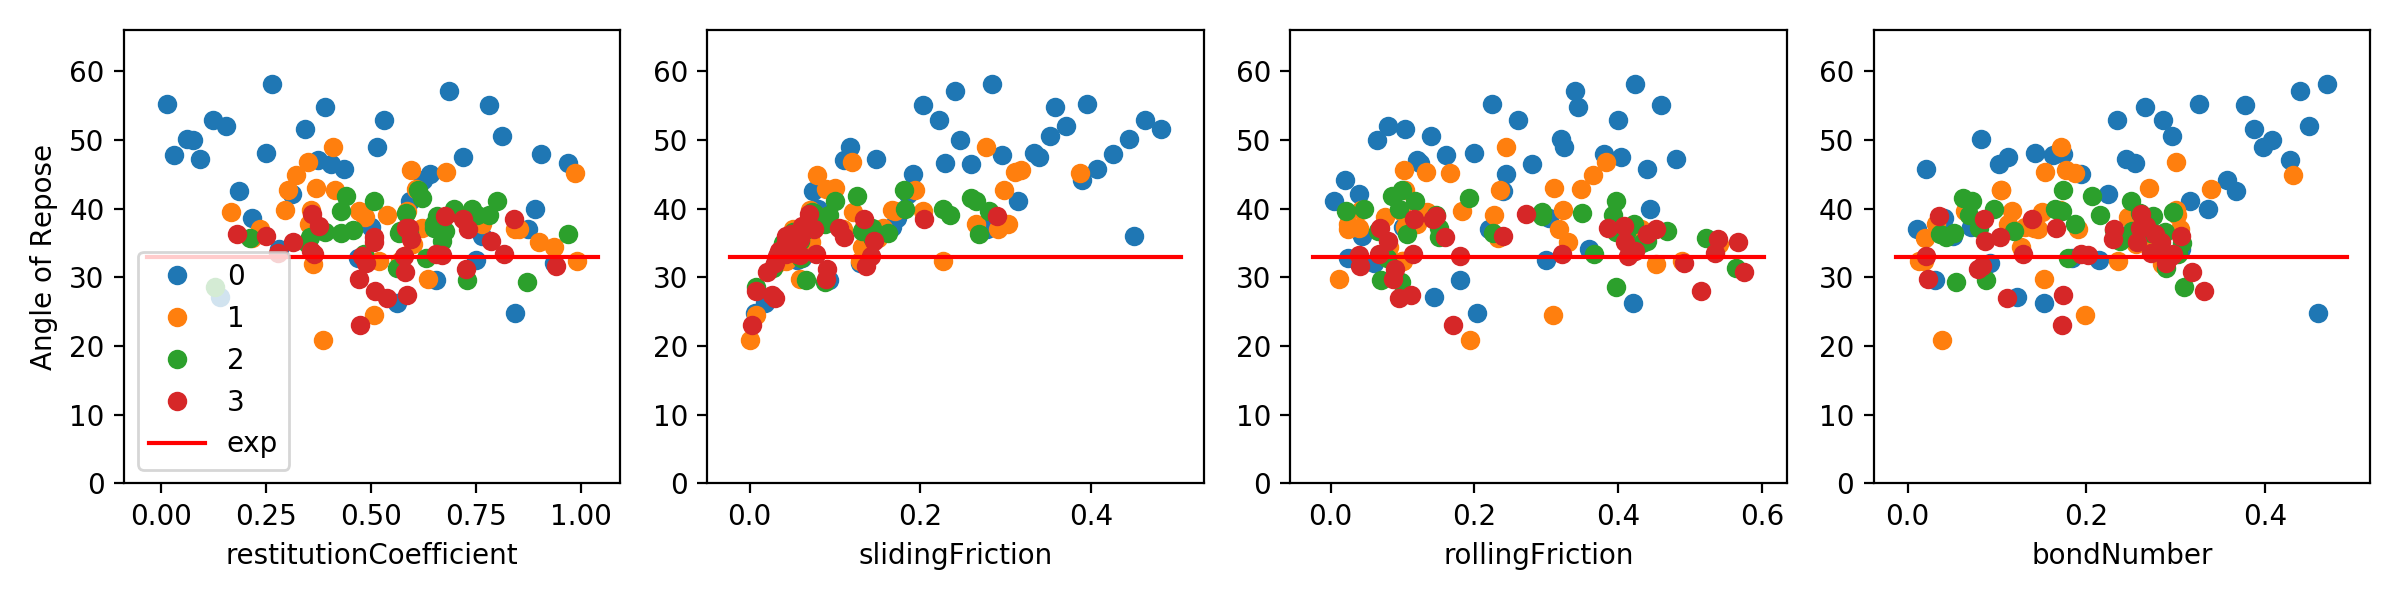
\includegraphics[scale=0.51]{ParametersObserver_Sand2.png}
    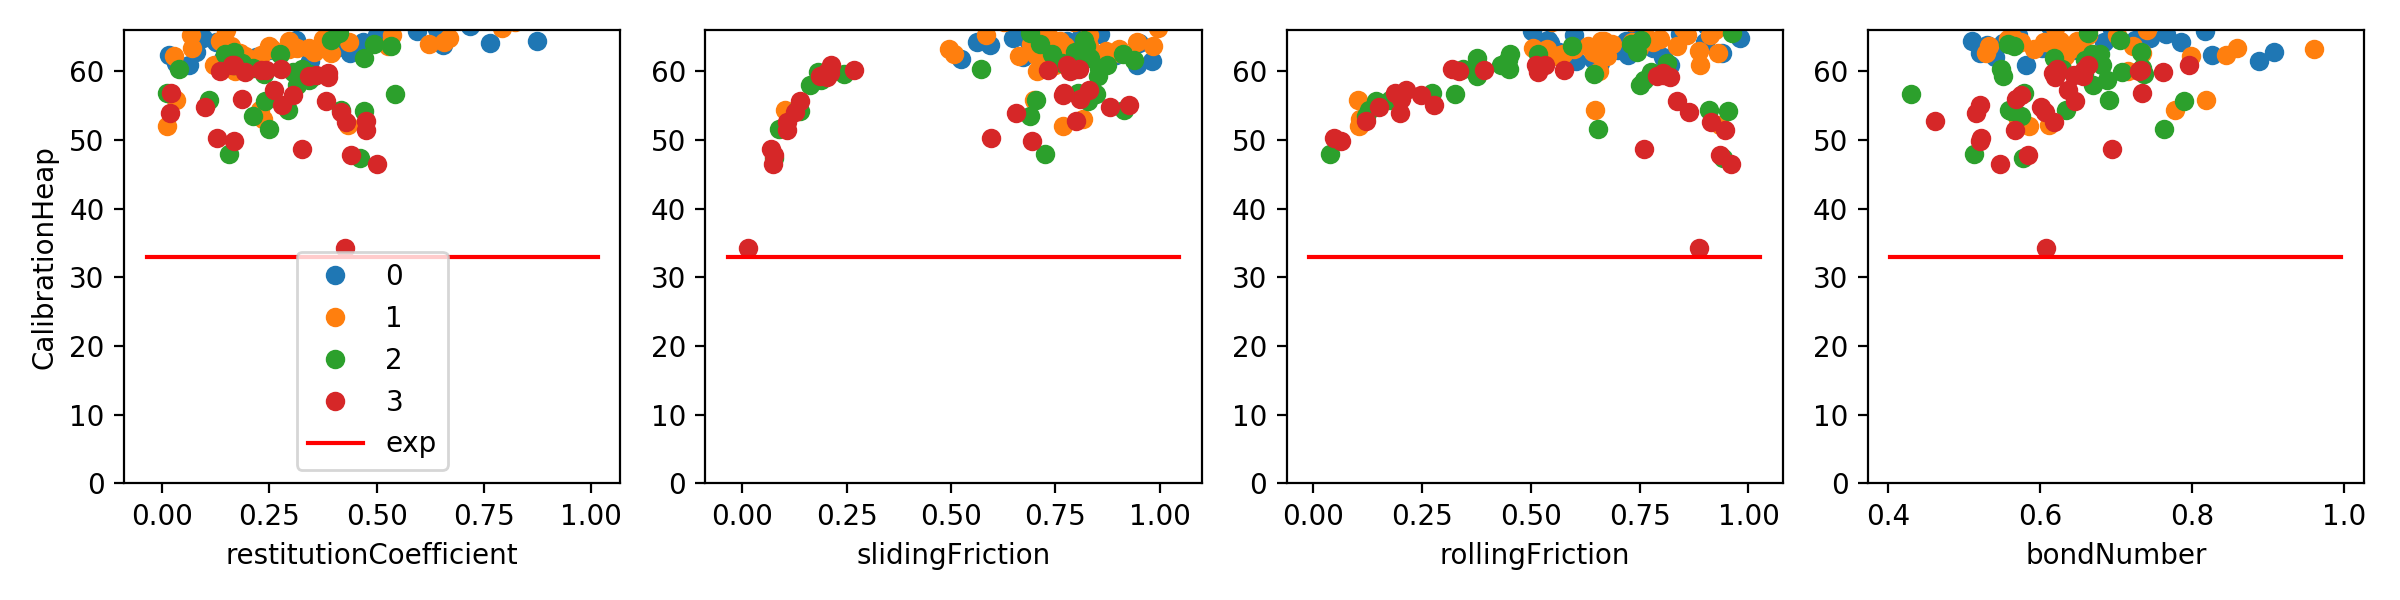
\includegraphics[scale=0.51]{ParametersObserver_Sand2_2.png}
    \caption{\textit{From top to bottom,} attempt 1, 2, and 3 at calibrating quartz sand with GL.\@ Scatter dots with different colors denote each iteration, and red line denotes experimental value.}\label{fig:QuartzGL}
\end{figure}

\begin{table}[ht]
    \centering
    \resizebox{\textwidth}{!}{%
    \begin{tabular}{c|ccccc}
    Attempt/Iter. & Restitution Coefficient & Sliding Friction & Rolling Friction & Bond number & Result AoR \\ \hline
    1.1 & 0.5703 & 0.0493 & 0.288 & 0.2448 & 31.6303 \\
    2.1 & 0.4688 & 0.0617 & 0.024 & 0.1836 & 32.8394 \\
    2.2 & 0.992 & 0.2261 & 0.0987 & 0.0126 & 32.3687 \\
    2.3 & 0.6307 & 0.0606 & 0.0787 & 0.1795 & 32.8670 \\
    2.4 & 0.4800 & 0.0321 & 0.413 & 0.2946 & 33.0521 \\
    3.1 & 0.0625 & 0.9444 & 0.82 & 0.5816 & 60.9714 \\
    3.2 & 0.0109 & 0.7683 & 0.1052 & 0.5853 & 52.0551 \\
    3.3 & 0.4604 & 0.0752 & 0.9406 & 0.5777 & 47.3408 \\
    3.4 & 0.427 & 0.0146 & 0.8872 & 0.6075 & 34.2227
    \end{tabular}%
    }\caption{Calibration results of sand with GL.}\label{table:resSandGL}
\end{table}
    
        
\subsection{GL discussion}

Throughout multiple calibration routines with GrainLearning, it is identified that the initial guessing range played a key role in the ability of GL to idenfity the correct set of micro-parameters.


\section{Supervised model evaluation}\label{section:supervisedPerformance}

In this section, the performance of the two supervised models, i.e., Neural Network and Random Forest, is investigated for limestone and quartz sand, respectively. 

\subsection{Limestone}

For limestone, 12 over 500,000 combinations of DEM input parameters processed by the ANN was a `valid' combination: the output of the ANN was $33\pm 0.01^{\circ}$. Meanwhile, with 2,500,000 million combinations processed by RF, 22 of them were valid combinations~-~however, many of them are closely similar with a minor difference in one of the micro parameters, and only nine are distinct. The valid combinations are described in table~\ref{table:EskalNN} and~\ref{table:eskalRF}, with figure~\ref{fig:EskalNNRF} illustrates the combinations and their respective output. Overall, the NN model has correctly identified three combinations, while the Random Forest model has 2. 


\begin{figure}[H]
    \centering
    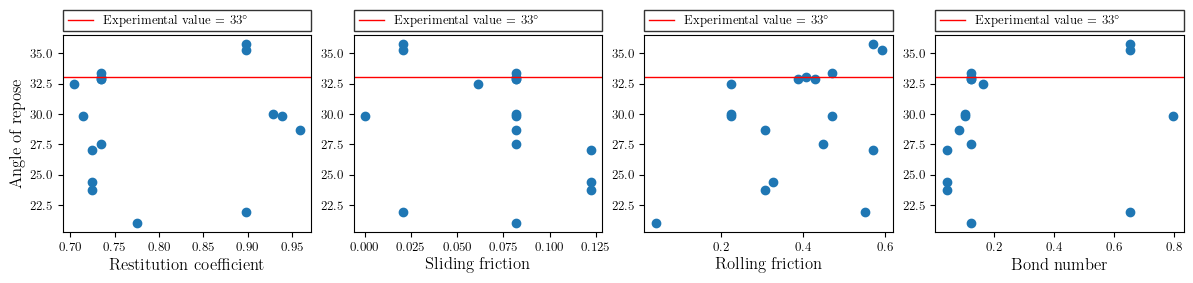
\includegraphics[scale=0.51]{rf_eskal.png}
    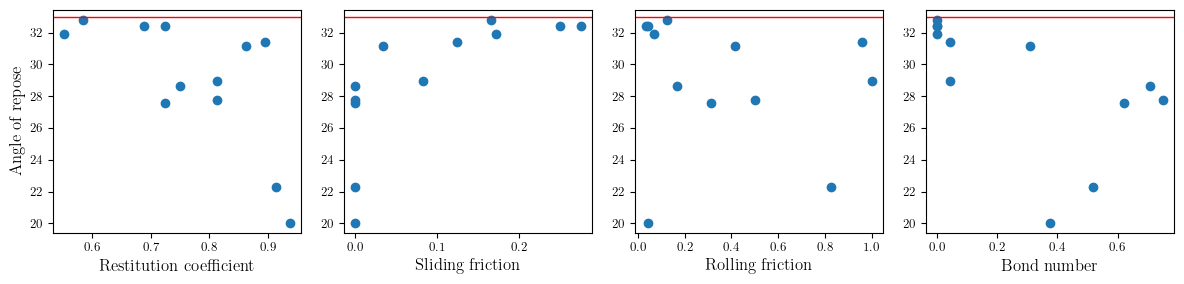
\includegraphics[scale=0.51]{nn_eskal.png}
    \caption{\textit{From top to bottom,} valid contact law parameters identified by Random Forest and Neural Network model for limestone, and their respective simulation results.}\label{fig:EskalNNRF}
\end{figure}

      
\begin{table}[H]
    \centering
    \resizebox{\textwidth}{!}{%
    \begin{tabular}{cccc|c}
    Restitution coefficient & Sliding friction & Rolling friction & Bond number & Angle of repose \\ \hline
    \textbf{0.6875} & \textbf{0.2500} & \textbf{0.0417} & \textbf{0} & \textbf{32.4263} \\
    0.7500 & 0 & 0.1667 & 0.7083 & 28.6156 \\
    \textbf{0.5833} & \textbf{0.1667} & \textbf{0.1250} & \textbf{0} & \textbf{32.7926} \\
    0.5517 & 0.1724 & 0.0690 & 0 & 31.9425 \\
    0.8125 & 0.0833 & 1.0000 & 0.0417 & 28.9393 \\
    \textbf{0.7241} & \textbf{0.2759} & \textbf{0.0345} & \textbf{0} & \textbf{32.3962} \\
    0.8958 & 0.1250 & 0.9583 & 0.0417 & 31.4044 \\
    0.8621 & 0.0345 & 0.4138 & 0.3104 & 31.1331 \\
    0.7241 & 0 & 0.3104 & 0.6207 & 27.5978 \\
    0.8125 & 0 & 0.5000 & 0.7500 & 27.7676 \\
    0.9138 & 0 & 0.8276 & 0.5172 & 22.2677 \\
    0.9375 & 0 & 0.0417 & 0.3750 & 20.0361
    \end{tabular}%
    }
    \caption{Valid contact law parameters identified by the NN model for limestone and their respective simulation results. }
    \label{table:EskalNN}
\end{table}
                
\begin{table}[H]
    \centering
    \resizebox{\textwidth}{!}{%
    \begin{tabular}{cccc|c}
    Restitution coefficient & Sliding friction & Rolling friction & Bond number & Angle of repose \\ \hline
    \textbf{0.7041} & \textbf{0.0612} & \textbf{0.2245} & \textbf{0.1633} & \textbf{32.4872} \\
    0.7245 & 0.1225 & 0.5714 & 0.0408 & 27.0585 \\
    \textbf{0.7347} & \textbf{0.0816} & \textbf{0.4082} & \textbf{0.1225} & \textbf{33.0331} \\
    0.7347 & 0.0816 & 0.4694 & 0.1225 & 33.3593 \\
    0.7755 & 0.0816 & 0.0408 & 0.1225 & 21.0172 \\
    0.8980 & 0.0204 & 0.5714 & 0.6531 & 35.7342 \\
    0.9286 & 0.0816 & 0.2245 & 0.1020 & 29.9625 \\
    0.9592 & 0.0816 & 0.3061 & 0.0816 & 28.6865 \\
    0.7143 & 0 & 0.4694 & 0.7959 & 29.8154
    \end{tabular}%
    }
    \caption{Valid contact law parameters identified by the RF model for limestone and their respective simulation results.}
    \label{table:eskalRF}
\end{table}


\subsection{Quartz Sand}

It is noteworthy that the quartz sand model was trained with less simulations compare to limestone model, with 322 DEM simulations. However, the performance of NN model when predicting the correct combinations that results in a static AoR of $33^{\circ}$: 4 out of 10 combinations are valid after verified by a full DEM simulation. Meanwhile, while the RF model predicts 20 different combinations, only 3 of them were valid~-~but interestingly, most of the combinations predict by RF model ranging very close to the experimental value, from  $29^{\circ}$ to  $31^{\circ}$. The number of combinations passed to NN and RF model for quartz sand is approximately the same as for limestone. 

\begin{figure}[H]
    \centering
    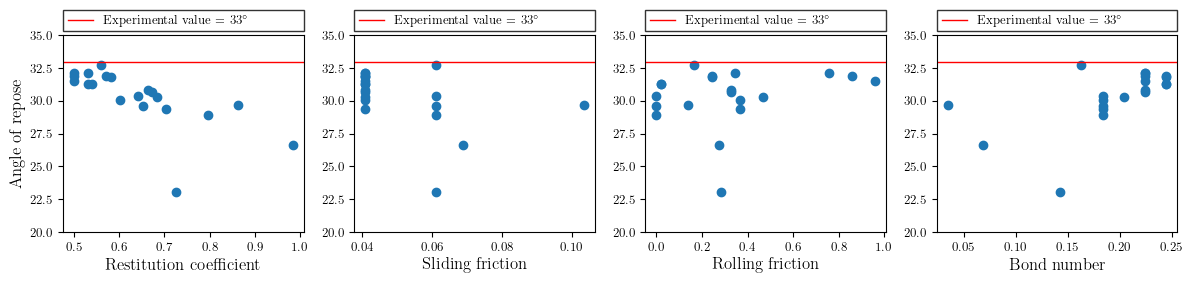
\includegraphics[scale=0.51]{rf_sand.png}
    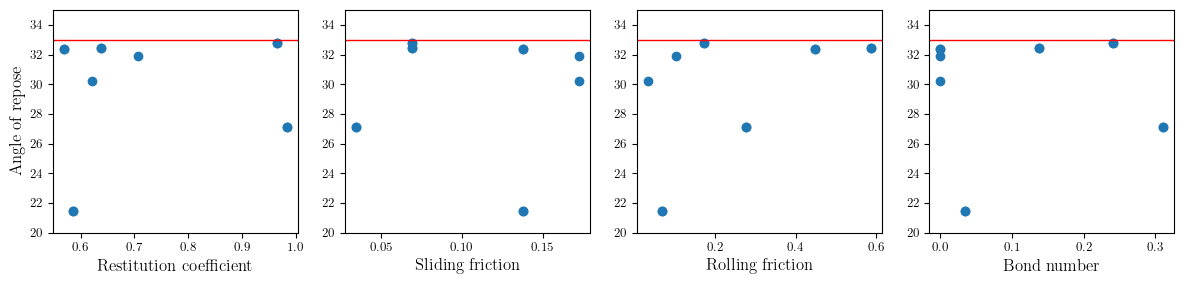
\includegraphics[scale=0.51]{nn_sand.png}
    \caption{\textit{From top to bottom,} valid contact law parameters identified by Random Forest and Neural Network model for quartz sand, and their respective simulation results.}\label{fig:SandNNRF}
\end{figure}

\begin{table}[H]
    \centering
    \resizebox{\textwidth}{!}{%
    \begin{tabular}{cccc|c}
    Restitution coefficient & Sliding friction & Rolling friction & Bond number & Angle of repose \\ \hline
    \textbf{0.5690} & \textbf{0.1379} & \textbf{0.4483} & \textbf{0} & \textbf{32.3822} \\
    0.7069 & 0.1724 & 0.1035 & 0 & 31.9092 \\
    0.6207 & 0.1724 & 0.0345 & 0 & 30.2535 \\
    \textbf{0.6379} & \textbf{0.0690} & \textbf{0.5862} & \textbf{0.1379} & \textbf{32.4170} \\
    0.5862 & 0.1379 & 0.0690 & 0.0345 & 21.4586 \\
    \textbf{0.9655} & \textbf{0.0690} & \textbf{0.1724} & \textbf{0.2414} & \textbf{32.7969} \\
    0.9828 & 0.0345 & 0.2759 & 0.3104 & 27.0953 \\
    0.5862 & 0.1379 & 0.0690 & 0.0345 & 21.4586 \\
    \textbf{0.9655} & \textbf{0.0690} & \textbf{0.1724} & \textbf{0.2414} & \textbf{32.7969} \\
    0.9828 & 0.0345 & 0.2759 & 0.3104 & 27.0953
    \end{tabular}%
    }
    \caption{Valid contact law parameters identified by the NN model for quartz sand and their respective simulation results.}\label{table:sandNN}
\end{table}

\begin{table}[H]
    \centering
    \resizebox{\textwidth}{!}{%
    \begin{tabular}{cccc|c}
    Restitution coefficient & Sliding friction & Rolling friction & Bond number & Angle of repose \\ \hline
    \textbf{0.5612} & \textbf{0.0612} & \textbf{0.1633} & \textbf{0.1633} & \textbf{32.7325} \\
    \textbf{0.5000} & \textbf{0.0408} & \textbf{0.7551} & \textbf{0.2245} & \textbf{32.1187} \\
    0.5000 & 0.0408 & 0.8571 & 0.2245 & 31.8814 \\
    \textbf{0.5306} & \textbf{0.0408} & \textbf{0.3469} & \textbf{0.2245} & \textbf{32.1125} \\
    0.6429 & 0.0612 & 0 & 0.1837 & 30.3771 \\
    0.5714 & 0.0408 & 0.2449 & 0.2449 & 31.8564 \\
    0.6020 & 0.0408 & 0.3674 & 0.1837 & 30.0461 \\
    0.5408 & 0.0408 & 0.0204 & 0.2449 & 31.2764 \\
    0.5000 & 0.0408 & 0.9592 & 0.2245 & 31.5459 \\
    0.5816 & 0.0408 & 0.2449 & 0.2449 & 31.8087 \\
    0.6531 & 0.0612 & 0 & 0.1837 & 29.6271 \\
    0.7041 & 0.0408 & 0.3674 & 0.1837 & 29.3786 \\
    0.6633 & 0.0408 & 0.3265 & 0.2245 & 30.8579 \\
    0.5306 & 0.0408 & 0.0204 & 0.2449 & 31.2787 \\
    0.6735 & 0.0408 & 0.3265 & 0.2245 & 30.6531 \\
    0.7959 & 0.0612 & 0 & 0.1837 & 28.9042 \\
    0.6837 & 0.0408 & 0.4694 & 0.2041 & 30.2650 \\
    0.7245 & 0.0612 & 0.2857 & 0.1429 & 23.0546 \\
    0.8621 & 0.1035 & 0.1379 & 0.0345 & 29.6629 \\
    0.9828 & 0.0690 & 0.2759 & 0.0690 & 26.6594
    \end{tabular}%
    }
    \caption{Valid contact law parameters identified by the RF model for quartz sand and their respective simulation results}
    \label{table:sandlRF}
\end{table}
    
\subsection{NN and RF model discussion}

Overall, the supervised models have demonstrated the ability to learn the contact law relationship of DPM for a specified materials. It is expected that the model would not has a high predition accuracy ($>70\%$) when being fed and process millions of combinations, with limited training data. And therefore, limitations of the model can be seen in some case, especially with quartz sand: the model


\section{Discussion}\label{section:discussion}

- GrainLearning has an inconsistent performance, especially when parameter ranges are specified too wide. Assume a calibration with GL cost 40 DEM simulations per iteration, for each bulk parameter it would be 7-8 iterations ~ 300 DEM simulations = > less DEM simulations, fully automatic, has been proven for more complex contact laws. 

- For limestone, the amount of DEM simulations used to train NN and RF are 485, and for quartz sand are 322. The numbers are slightly higher than GL, but the performance are more robust from a small experiment: Produces multiple valid combinations per bulk parameter, therefore easier to identify the correct one by comparision with other bulk parameter's combinations. 

- Limitations of RF: has not been tested against complex contact laws

